\newpage
\section{Introduction}

Mapless navigation with deep reinforcement learning is an innovative approach to autonomous navigation that aims to empower robotic systems with the ability to traverse and explore their environments without relying on pre-built maps or explicit mapping processes. The motivation behind this project is to reduce the dependency on prior knowledge of the environment and enable more adaptive navigation in dynamic and unpredictable settings. The project has successfully demonstrated that, by employing deep reinforcement learning, robots can acquire intelligent behaviours for navigating simple cluttered environment. The code and demonstration videos are available on \url{https://github.com/MinghongAlexXu/final-year-proj}.

The report is organised as follows: 
In Section \ref{subsec:spec}, the project specification is given.
Section \ref{subsec:drl} and \ref{subsec:mapless-navi} is the background on deep reinforcement learning and mapless navigation.
Section \ref{sec:literature} is the literature survey on DRL and mapless navigation.
Section \ref{sec:impact} details the industrial relevance, real-world applicability, and scientific impact.
Section \ref{sec:theory} explains the theories used in this project.
The project's software library design is given in Section \ref{sec:design}.
Section \ref{sec:method} details the experimental method used in this project.
Section \ref{sec:results} reports the results.
Section \ref{sec:discussion} provides a discussion of the results and DRL, in general.
Section \ref{sec:reflection} reflects on this project-based learning.
Finally, Section \ref{sec:conclusion} concludes the report.



\subsection{Project Specifications} \label{subsec:spec}

The goal of this project is to gain insights into deep reinforcement learning by i) implementing the algorithm and a simulation environment, ii) training policies, and iii) performance evaluation \cite{ref:spec-report}. The engineering tasks of this project mainly consists of implementing the algorithm and the environment, as well as training the policies. Therefore, this is a software engineering project that aims to enable research work in the field of deep reinforcement learning.

For this project, mapless navigation was chosen as a case study for deep reinforcement learning. From the perspective of deep reinforcement learning, any task that it can solve is nothing more than a dataset described by a Markov decision process. Therefore, any task that can be formulated as a Markov decision process is a potential candidate for this project. Initially, quadrupedal locomotion learning was considered, but due to its high engineering complexity, which is close to the level of doctoral research, the idea was eventually abandoned in favour of mapless navigation on account of time constraints.

Mapless navigation is a robotic task that requires the robot's motion planner to navigate the robot to a target location without relying on a map, while avoiding obstacles along the way. In the framework of deep reinforcement learning, the motion planner here can simply be modelled by a policy neural network. The performance of the motion planner can be gradually improved by updating its model weights according to a predefined reward signal through training using reinforcement learning algorithms.

The main line of this project was planned step by step. The first step was reading the literature to get more familiar with the algorithms. The next step was to implement these algorithms and group them as a software package. The following step developed a simulation training environment for mapless navigation. In the final step, the algorithms were combined with the environment to train policies and gradually increase the complexity of the environment depending on the performance at each stage. The focus is on gaining a deeper understanding of reinforcement learning through the above process.

The project objectives are hence three-fold:
\begin{enumerate}[label=\arabic*), nosep, leftmargin=*]
    \item Implement deep reinforcement learning algorithms and a simulated mapless navigation training environment.
    \item Train policies that move an agent towards a target on a level ground with no obstacles.
    \item Policy training for the case with obstacles.
\end{enumerate}
Tasks and deliverables encompass both research and engineering efforts. They are detailed below which will satisfy the objectives set out. The verification metrics are given in the Table \ref{table:specifications-verification-matrix}.

\begin{enumerate}[label=Task \arabic*{,}, leftmargin=*]
    \item \textbf{literature survey}: This task will review the recent work on mapless navigation that use deep reinforcement learning. The outcome will be a brief report on the topic (D.1).
    \item \textbf{library implementation}: State-of-the-art deep reinforcement learning algorithms, including DDPG, TD3, and SAC, will be implemented and grouped together as a Python package (D.2).
    \item \textbf{training environment implementation}: A flat floor indoor environment will be implemented in the Gazebo Classic simulator. The environment can be completely obstacle-free, may contain some fixed obstacles, or may include randomly moving obstacles, depending on the performance of the training at each stage to gradually increase the complexity of the environment (D.3).
    \item \textbf{training near-optimal policies}: The policies will be trained by using the D.2 and D.3 until they reach their near-optimal point (the episodic return stops increasing). The performance of the near-optimal policies will be illustrated by episodic return curves and visualised in demonstration videos and a rendering program (D.4).
    \item \textbf{report insights gained}: The research outcomes will be reported in the project final report (D.5).
\end{enumerate}

\begin{enumerate}[label=D. \arabic*:, leftmargin=*]
    \item Brief report on the recent work on mapless navigation using deep reinforcement learning.
    \item A library implementation.
    \item A training environment implementation.
    \item Trained policies with illustration and visualisation of their performance.
    \item Report the insights on deep reinforcement learning gained through experience.
\end{enumerate}

\begin{table}[htbp]
   \centering
   \caption{Specifications verification metrics \cite{ref:spec-report}}
   \label{table:specifications-verification-matrix}
   \begin{tblr}{
      width=0.9\linewidth,
      colspec={|X|X|},
      hlines,
   }
   Specification & Verification \\
   \hline
   Implement state-of-the-art deep reinforcement learning algorithms. & Test on baseline environments. \\
   Train policies in an empty world. & Robot can reach the target position. \\
   Train policies in an indoor environment filled with obstacles. & Robot can reach the target position and not collide with obstacles. \\
   \end{tblr}
\end{table}

The project was expected to take seven months to complete. To ensure the success of this project, a timeline was established to keep track of the progress of each task. The timeline included specific milestones and deadlines for each task, as well as regular meetings to discuss the progress and make any necessary adjustments. The timeline was partially represented as a Gannt chart. See Appendix \ref{appx:plan}.



\subsection{Deep reinforcement learning} \label{subsec:drl}

Reinforcement learning is a machine learning paradigm that optimises a function implementing a policy for a specific agent in a particular environment through trial-and-error experiences~\cite{ref:spinning-up}. Deep reinforcement learning (DRL) is a type of reinforcement learning that uses deep neural networks, artificial neural networks (ANN) composed of multiple layers, for function approximation~\cite{ref:dqn}.

\begin{figure}[htbp]
\centering
\includesvg[width=0.5\textwidth]{agent-env-interaction}
\caption{Typical model for reinforcement learning paradigm \cite{ref:spec-report}}
\label{fig:agent-env-interaction}
\end{figure}

As illustrated in Figure \ref{fig:agent-env-interaction}, the agent learns to act by iteratively observing its own state and the surrounding environment, taking actions, and receiving rewards for those actions. At each time step $t$, with a given state $s_t \in S$, the agent takes an action $a_t \in A$ according to its policy $\pi \colon S \to A$, receives a reward $r(s_t, a_t)$, and transitions to a new state based on $p(s_{t+1}|s_t, a_t)$. This sequential decision-making process is formally modelled as a Markov decision process (MDP), which is a quadruple $\langle S, A, p, r \rangle$, where:
\begin{itemize}
\item $S$, the state space, is a set of all valid states,
\item $A$, the action space, is a set of all valid actions,
\item $p \colon S \times A \to \Delta S$, a transition probability function representing the probability of transitioning to the next state if a specific action is taken in the current state,
\item $r \colon S \times A \to \mathbb{R}$, a reward function generating a reward signal.
\end{itemize}
The objective is to find an optimal policy that maximises the cumulative reward accumulated through each state.
\begin{displaymath}
\max_{\pi} \sum_{t} \mathbb{E}_{s_t \sim p_\pi, a_t \sim \pi} \left[ r(s_t,a_t) \right]
\end{displaymath}

Numerous algorithms have been proposed to address this problem, which can be broadly divided into:
\begin{itemize}
\item model-based, which utilises an environment model predicting state transitions,
\item model-free, which is based on the common case where the model is not available to the agent.
\end{itemize}
Figure \ref{fig:taxonomy-of-algorithms} presents a rough algorithm classification and representative algorithms under each classification. Note that some algorithms may possess multiple attributes.
\begin{figure}[htbp]
\centering
\includesvg[pretex=\tiny,width=\textwidth]{taxonomy-of-algorithms}
\caption{A non-exhaustive taxonomy of reinforcement learning algorithms \cite{ref:spinning-up}}
\label{fig:taxonomy-of-algorithms}
\end{figure}

The two main approaches for model-free algorithms are Policy Optimisation and Q-Learning. Policy Optimisation is stable and reliable but sample inefficient, while Q-Learning is sample efficient but more likely to fail due to its unprincipled nature. Of the three state-of-the-art model-free DRL algorithms, PPO, TD3, and SAC, PPO uses only the first approach, while the latter two are a mixture of both approaches.

In model-based DRL, the agent learns or is given a model of the environment's dynamics and uses this model for planning and decision-making. With a learned environment model, the agent can plan its actions by simulating different trajectories or sequences of actions in the model. Various planning algorithms, such as Monte Carlo Tree Search (MCTS) or Model Predictive Control (MPC), can be used to find the best action sequence. By explicitly exploiting a model of the environment, model-based DRL has the potential to achieve better sample efficiency and generalisation compared to model-free methods \cite{ref:model-based-survey}. However, it also faces challenges, including the difficulty of learning accurate environment models and the computational complexity of planning algorithms.



\subsection{Mapless navigation} \label{subsec:mapless-navi}

DRL can be applied to accomplish robotic tasks, such as mapless navigation. Mapless navigation is a type of motion planning task that enable a robot to navigate its environment without relying on pre-built maps or prior knowledge of the area~\cite{ref:virtual2real-drl}. Instead, the system utilises various sensors, such as cameras, LiDAR, or other depth-sensing devices, to perceive its surroundings in real-time and plan its motion accordingly.

\begin{figure}[htbp]
\centering
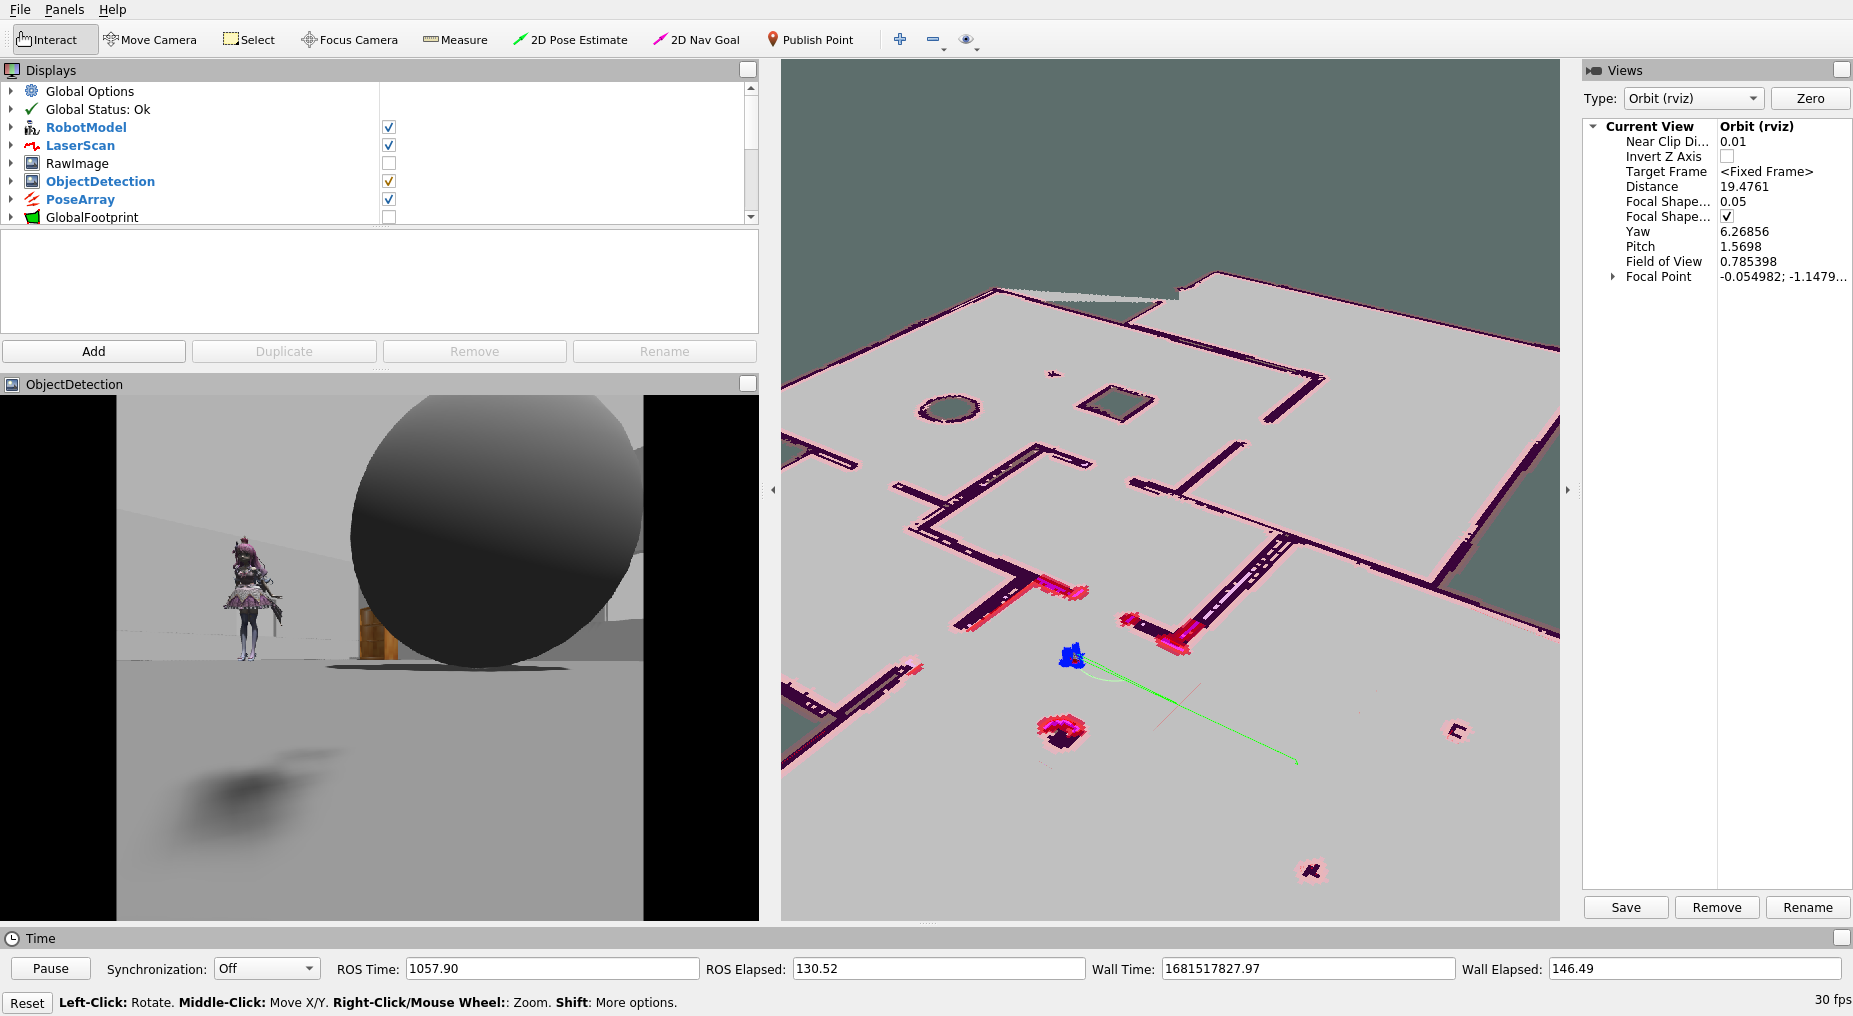
\includegraphics[width=\textwidth]{SLAM.png}
\caption{SLAM-based autonomous navigation in Gazebo Classic visualised with RViz.}
\label{fig:slam}
\end{figure}

Building and updating global obstacle maps is time-consuming and relies on precise depth sensors. Figure \ref{fig:slam} shows autonomous navigation after building a map using SLAM in a simulation environment. DRL can offer a relatively low-cost solution to this task with the help of emerging localisation methods such as Wi-Fi localisation. Moreover, the mapless navigate ability is particularly useful in situations where maps are unavailable, outdated, or impractical, such as in unpredictable terrains or rapidly changing environments.
